%%%%%%%% ICML 2025 EXAMPLE LATEX SUBMISSION FILE %%%%%%%%%%%%%%%%%

\documentclass{article}

% Recommended, but optional, packages for figures and better typesetting:
\usepackage{microtype}
\usepackage{graphicx}
\usepackage{subfigure}
\usepackage{booktabs} % for professional tables

% hyperref makes hyperlinks in the resulting PDF.
% If your build breaks (sometimes temporarily if a hyperlink spans a page)
% please comment out the following usepackage line and replace
% \usepackage{icml2025} with \usepackage[nohyperref]{icml2025} above.
\usepackage{hyperref}


% Attempt to make hyperref and algorithmic work together better:
\newcommand{\theHalgorithm}{\arabic{algorithm}}

% Use the following line for the initial blind version submitted for review:
\usepackage{icml2025}

% If accepted, instead use the following line for the camera-ready submission:
% \usepackage[accepted]{icml2025}

% For theorems and such
\usepackage{amsmath}
\usepackage{amssymb}
\usepackage{mathtools}
\usepackage{amsthm}

\usepackage{enumitem}

\newcommand{\p}[0]{\mathbf{p}}
\newcommand{\x}[0]{\mathbf{x}}
\newcommand{\w}[0]{\mathbf{w}}
\renewcommand{\v}[0]{\mathbf{v}}
\newcommand{\z}[0]{\mathbf{z}}
\newcommand{\Z}[0]{\mathbf{Z}}
\newcommand{\X}[0]{\mathbf{X}}

\newcommand{\R}[0]{\mathbb{R}}
\newcommand{\E}[0]{\mathbb{E}}
\newcommand{\V}[0]{\mathcal{V}}
\newcommand{\conj}[1]{ {\overline{#1}} }
\newcommand{\comp}[1]{ {\overline{#1}} }
\newcommand{\inprod}[1]{\langle#1\rangle}
\newcommand{\norm}[1]{\left\lVert#1\right\rVert}
\newcommand{\horline}{\noindent\rule{\linewidth}{0.4pt}}
\newcommand{\paren}[1]{\left( #1 \right)}


% if you use cleveref..
\usepackage[capitalize,noabbrev]{cleveref}

%%%%%%%%%%%%%%%%%%%%%%%%%%%%%%%%
% THEOREMS
%%%%%%%%%%%%%%%%%%%%%%%%%%%%%%%%
\theoremstyle{plain}
\newtheorem{theorem}{Theorem}[section]
\newtheorem{proposition}[theorem]{Proposition}
\newtheorem{lemma}[theorem]{Lemma}
\newtheorem{corollary}[theorem]{Corollary}
\theoremstyle{definition}
\newtheorem{definition}[theorem]{Definition}
\newtheorem{assumption}[theorem]{Assumption}
\theoremstyle{remark}
\newtheorem{remark}[theorem]{Remark}
\newtheorem{example}[theorem]{Example}

% Todonotes is useful during development; simply uncomment the next line
%    and comment out the line below the next line to turn off comments
%\usepackage[disable,textsize=tiny]{todonotes}
\usepackage[textsize=tiny]{todonotes}


% The \icmltitle you define below is probably too long as a header.
% Therefore, a short form for the running title is supplied here:
\icmltitlerunning{Decision focused meta-learning}

\begin{document}

\twocolumn[
\icmltitle{Decision focused meta-learning}

% It is OKAY to include author information, even for blind
% submissions: the style file will automatically remove it for you
% unless you've provided the [accepted] option to the icml2025
% package.

% List of affiliations: The first argument should be a (short)
% identifier you will use later to specify author affiliations
% Academic affiliations should list Department, University, City, Region, Country
% Industry affiliations should list Company, City, Region, Country

% You can specify symbols, otherwise they are numbered in order.
% Ideally, you should not use this facility. Affiliations will be numbered
% in order of appearance and this is the preferred way.
\icmlsetsymbol{equal}{*}

\begin{icmlauthorlist}
\icmlauthor{Rares Cristian}{mit}
\end{icmlauthorlist}

\icmlaffiliation{mit}{Operations Research Center, Massachusetts Institute of Technology, Cambridge, MA, USA}
% \icmlaffiliation{comp}{Company Name, Location, Country}
% \icmlaffiliation{sch}{School of ZZZ, Institute of WWW, Location, Country}

\icmlcorrespondingauthor{Rares Cristian}{raresc@mit.edu}

% You may provide any keywords that you
% find helpful for describing your paper; these are used to populate
% the "keywords" metadata in the PDF but will not be shown in the document
\icmlkeywords{end-to-end learning, task-learning, optimization, ICML}

\vskip 0.3in
]

% this must go after the closing bracket ] following \twocolumn[ ...

% This command actually creates the footnote in the first column
% listing the affiliations and the copyright notice.
% The command takes one argument, which is text to display at the start of the footnote.
% The \icmlEqualContribution command is standard text for equal contribution.
% Remove it (just {}) if you do not need this facility.

%\printAffiliationsAndNotice{}  % leave blank if no need to mention equal contribution
\printAffiliationsAndNotice{\icmlEqualContribution} % otherwise use the standard text.

\begin{abstract}
This is a great concise abstract :)
\end{abstract}

\section{Introduction}
\label{sec:intro}

Real-world decision-making is often faced with uncertainty, such as inventory allocation in warehouse networks, scheduling electricity generation, shortest path planning in traffic and more. In practice, these problems are often split into two stages, each dealt with by separate teams: forecasting and optimization. These constitute \emph{predict-then-optimize} approaches. For example, first one machine learning (ML) model is trained to predict demand of electricity, and second, this prediction is fed into an optimization problem to schedule the electricity generation. Such an approach makes the assumption that better forecasts implies better decisions which, surprisingly at first glance, is often not the case. If one makes perfect predictions, then  this indeed results in optimal decisions. However, this is unlikely to ever happen. Moreover, the prediction stage objective (to minimize mean-squared prediction error) is not directly aligned with the decision-making second stage. For example, when predicting demand for various items across a network of warehouses, the loss function essentially treats each warehouse independently. However, the final decision of how to allocate inventory and how to optimally fulfill demand depends globally on interactions across all warehouses. In such a predict-then-optimization framework, the prediction stage is therefore unaware of these complex interactions, leading to suboptimal decisions.

The area of \emph{decision-focused learning} (DFL) aims to build ML predictive models that directly minimize decision-based loss. In short, DFL methods train predictive models that lead to the best decision, the true ultimate goal. Such methods have shown considerable performance improvements over predict-then-optimize approaches, consistently leading to better decision-making. However, the specific tailoring of DFL methods to the decision-making task is also one reason that is keeping it from more widespread adoption. DFL methods train a model for a specific formulation of an optimization problem, for example a fixed network of warehouses with fixed shipping costs or other fixed operational costs. In practice, these parameters of the optimization problem are not fixed and can often change over time. This drawback of DFL methods lacking study into their generalization to new tasks is also addressed in a recent survey \cite{mandi2024decision}. 

In this paper, we propose a general framework and network architecture that allows for decision-focused learning across distributions of tasks. 

\subsection{Related literature}

\subsection{Background and the decision-focused learning framework}

Finally, we formally introduce the overarching problem of contextual optimization which we will tackle from different viewpoints in the following chapters. As a running example, we will consider an electricity-scheduling problem.

\begin{itemize}[leftmargin=*]
    \item \emph{Decisions and constraints}. The goal of the problem is to make (optimal) decisions $\v$ in a convex feasible region $\mathcal{V}(\p) \subset \R^d$ in dimension $d$. The decision space is parameterized by some vector $\p$ corresponding to different parameters of the problem. This $\p$ defines a task. For example, 
    \item \emph{Uncertainty}. We must take decisions in the face of uncertainty, specifically some random variable $\Z$. For example, $\Z \in \R^{24}_{+}$ denoting the demand of electricity at each hour.
    \item \emph{Context}. The outcome of the random variable $\Z$ can depend on contextual information $\x$. For example, demand $\Z$ can depend on temperature, price, time information like whether it's a weekend or a holiday, and so on. All of this contextual information is embedded in the features observation $\x$. Given an observation of features $\x$, the random variable has conditional distribution $\Z | \x$. We will also say that realizations $\x$ is distributed according to the random variable $\mathbf{X}$.
    \item \emph{Cost}. After we make a decision $\v$, we observe a \emph{realization} (or a \emph{sample}) of $\z \sim \Z|\x$. For instance, after creating the electricity schedule $\v$, we observe the true demand at the end of the day. We then incur a cost $c_{\p}(\v, \z)$ where again $\p$ is a parameterization of the cost function. For instance, in the electricity-scheduling problem, $\p$ can correspond to the price of electricity, a constant value in the scheduling problem, but which may change from one instance to another (such as from one day to the next, prices may change and so does the scheduling problem).
\end{itemize}
The final goal is to make a decision $\v \in \mathcal{V}(\p)$ which minimizes the expected cost
\begin{equation}
    \mathbb{E}_{\z \sim \Z|\x}[c_{\p}(\v, \z)].
\end{equation}
This is a difficult problem in practice since the distributions $\Z$ and $\Z|\x$ are unknown. Instead, we will assume that we have access to data:
\begin{itemize}
    \item \emph{Data.} We assume we are given a dataset of $N$ points $(\x_n, \z_n), n = 1,\dots,N$ with realization  $\z_n \sim \Z|\x_n$. We are also given a set $\p_1, \dots, \p_M$ of different parameterizations of the optimization problem. For the sake of analysis, suppose parameters $\p$ are distributed according to $\mathbf{P}$.
\end{itemize}

% \begin{example}[Newsvendor]
% \label{eq:newsvendor-example1}
% As a simple example to illustrate the problem, consider the traditional single-item newsvendor problem \cite{arrow1951optimal} with no constraints. In particular, we make a decision $v \in \R_+$ for the amount of inventory of a single item to place in a store. The random variable $Z \in \R_+$ corresponds to the random demand for the item. For simplicity, assume no additional features $\x$. The cost of storing $v$ against demand $z$ is 
% \begin{equation}
% \label{eq:newsvendor-1}
% c(v,z) = h \cdot (v - z)^+ - b \cdot (z - v)^+    
% \end{equation}
% where $y^+$ denotes the positive part of $y$: $y^+ = \max\{y, 0\}$. The constants $h$ and $b$ refer to holding and backorder costs. Often, $b > h$ since leaving demand unfulfilled is overall more costly (think of this is a lost opportunity cost). Given full information on demand $\Z$, the optimal allocation policy is to stock $v=v^*$ as the $(b / (h + b))^{th}$ quantile of demand  $\Z$. However, over-stocking $v = v^* + \delta$ has a lower expected cost than equally under-stocking $v = v^* - \delta$. This is because of the imbalance in the objective $c(v,z)$.
% \end{example}

The decision-focused learning problem we will focus on is to learn a model, generally a neural network, $f(\x; \p)$ so that the corresponding decisions have minimum cost under task $\p$. That is, given a point prediction $f(\x; \p)$, we take the decision $v^*_{\p}(f(\x; \p))$ corresponding to the optimal decision under a task parameterized by $\p$ and forecast of $f(\x; \p)$:
\begin{equation}
    v^*_{\p}(f(\x; \p)) = \arg\min_{\v \in \V(\p)} c_{\p}(\v, f(\x; \p)).
\end{equation}
Then, the decision $v^*_{\p}(f(\x; \p))$ is confronted by the true realizations of $\z \sim \Z|\x$ and incur expected cost 
\begin{equation}
    \E_{\z \sim \Z|\x} \left[ c_{\p}(v^*_{\p}(f(\x;\p)), \z) \right].
\end{equation}
% \begin{remark}
%     At first glance, from a prediction standpoint, the presence of both parameters $\p$ and of context $\x$ as separate information may seem unnecessary. That is, one could view the combination of $\x$ and $\p$ as a joint random variable and use this directly as input to a forecasting model $f$. Then, the neural network would learn the relevant relationship between context $\x$ and task $\p$. However, 
% \end{remark}
Overall, the learning task given empirical data is given by
\begin{equation}
    \min_{f} \sum_{m=1}^M \sum_{n=1}^N c_{\p_m}(v^*_{\p_m}(f(\x_n; \p_m), \z_n)),
\end{equation}
to learn a single model $f$ that can generalize across tasks. Existing decision-focused learning methods focus on various aspects of this problem for a single fixed task $\p$ and do not consider possible changes in $\p$. One possible solution is, for each $\p$, to train a new model through decision-focused learning specifically for the new instance of $\p$. However in practice, the task $\p$ can change often, such as for the inventory problem discussed above as shipping costs change constantly. We will present and discuss several methods for the cross-task problem in the following section.

\paragraph{Why not distributional forecasts?} Instead of making a point forecast $f(\x; \p)$, we might instead wish to train a network to make a distributional forecast. Such a method may be more interpretable, however it can also be prohibitively expensive as we would need to solve a stochastic optimization problem to evaluate the decisions resulting from the distributional forecast. Much of the decision-focused learning literature also focuses on point forecasts \cite{}, \cite{}, \cite{}. Finally, point forecasts are sufficient for linear objective functions: by linearity it suffices to make a point forecast of the mean of the distribution of each objective coefficient.

\section{Meta learning for optimization problems}

\begin{figure*}[t]
    \centering
    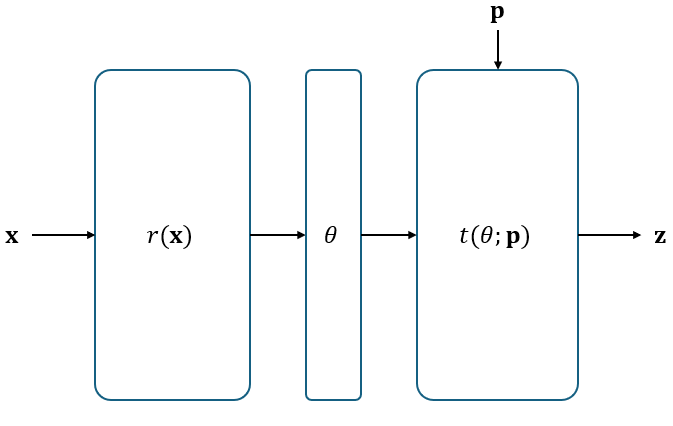
\includegraphics[width=0.5\linewidth]{images/cross_task_arch.png}
    \caption{Caption}
    \label{fig:architecture}
\end{figure*}

We begin by distinguishing our setting of meta-learning for optimization-style problems compared to more traditional meta-learning problems.
\emph{The ground-truth distribution $\Z|\x$ is independent of the task}. For instance, demand of items is independent of changes in shipping cost (changes in the task). For more traditional meta-learning problems, such as few-shot image classification, the target distribution fundamentally changes (like predicting a new class of objects). 

This observation lets us cleanly split the problem in two. Suppose we knew the distribution $\Z|\x$. Then, the optimal point forecast depends only on $\Z|\x$ and the specific task $\p$. Moreover, $\Z|\x$ depends only on a function of $\x$ and not of $\p$. Therefore, we propose to design the architecture of $f(\x; \p)$ as a composition of two models: (1) a representation learner $r(\x)$ that learns a representation $\theta$ of $\Z|\x$ and (2) a task learner $t(\theta, \p)$ meant to learn the correct point forecast. Then, $f(\x; \p) = t(r(\x); \p)$.

% We now analyze the problem of the task-learner from an optimization standpoint. Suppose $\theta$ is (unrealistically) equal to the distribution $\Z|\x$. Then, how does the optimal $t(\Z|\x; \p)$ behave as we change $\p$ and $\Z|\x$? 

% \begin{enumerate}
%     \item {concatenating task and representation.} As a simple baseline, we can construct $t(\theta; \p)$ to take as input the concatenation of the learned representation $\theta$ and the task $\p$. The network itself can be a multi-layer feed-forward network. 
%     \item \emph{task-learner as hypernetwork.}  Taking inspiration from the 
% \end{enumerate}

See Figure \ref{fig:architecture}.


\newpage
\section*{Impact Statement}
This paper presents work whose goal is to advance the field of 
Machine Learning. There are many potential societal consequences 
of our work, none which we feel must be specifically highlighted here.

\bibliography{bib}
\bibliographystyle{icml2025}

%%%%%%%%%%%%%%%%%%%%%%%%%%%%%%%%%%%%%%%%%%%%%%%%%%%%%%%%%%%%%%%%%%%%%%%%%%%%%%%
%%%%%%%%%%%%%%%%%%%%%%%%%%%%%%%%%%%%%%%%%%%%%%%%%%%%%%%%%%%%%%%%%%%%%%%%%%%%%%%
% APPENDIX
%%%%%%%%%%%%%%%%%%%%%%%%%%%%%%%%%%%%%%%%%%%%%%%%%%%%%%%%%%%%%%%%%%%%%%%%%%%%%%%
%%%%%%%%%%%%%%%%%%%%%%%%%%%%%%%%%%%%%%%%%%%%%%%%%%%%%%%%%%%%%%%%%%%%%%%%%%%%%%%
\newpage
\appendix
\onecolumn
\section{You \emph{can} have an appendix here.}

You can have as much text here as you want. The main body must be at most $8$ pages long.
For the final version, one more page can be added.
If you want, you can use an appendix like this one.  

The $\mathtt{\backslash onecolumn}$ command above can be kept in place if you prefer a one-column appendix, or can be removed if you prefer a two-column appendix.  Apart from this possible change, the style (font size, spacing, margins, page numbering, etc.) should be kept the same as the main body.
%%%%%%%%%%%%%%%%%%%%%%%%%%%%%%%%%%%%%%%%%%%%%%%%%%%%%%%%%%%%%%%%%%%%%%%%%%%%%%%
%%%%%%%%%%%%%%%%%%%%%%%%%%%%%%%%%%%%%%%%%%%%%%%%%%%%%%%%%%%%%%%%%%%%%%%%%%%%%%%


\end{document}


% This document was modified from the file originally made available by
% Pat Langley and Andrea Danyluk for ICML-2K. This version was created
% by Iain Murray in 2018, and modified by Alexandre Bouchard in
% 2019 and 2021 and by Csaba Szepesvari, Gang Niu and Sivan Sabato in 2022.
% Modified again in 2023 and 2024 by Sivan Sabato and Jonathan Scarlett.
% Previous contributors include Dan Roy, Lise Getoor and Tobias
% Scheffer, which was slightly modified from the 2010 version by
% Thorsten Joachims & Johannes Fuernkranz, slightly modified from the
% 2009 version by Kiri Wagstaff and Sam Roweis's 2008 version, which is
% slightly modified from Prasad Tadepalli's 2007 version which is a
% lightly changed version of the previous year's version by Andrew
% Moore, which was in turn edited from those of Kristian Kersting and
% Codrina Lauth. Alex Smola contributed to the algorithmic style files.
